\chapter{Project execution}

In the following chapter, we review the execution of the High Level Assembler Plugin software project. 
We analyze the problem difficulty, break it into tasks and estimate time requirements of particular tasks.
We further describe the team and work organization.

\section{Collaboration}
The team consists of five members. As the collaboration within the team is essential for successful completion of the project, we use a variety of means and methods to achieve this. 

Our team works with agile software development. To aid this, we use a visual process management system called Kanban. Our team meets every week with our supervisor at stand-ups and discusses the current status of particular tasks with their owners, reviews progress and plans work for the next week.

For communication between team members, we use an online tool --- Slack.

\section{Milestones and work packages}
We analyzed the problem and split it into several milestones and work packages. At the time of writing this document,  the milestone \hyperref[milestone_preview]{Preview} has been reached. Therefore, there is currently a working prototype, and some of the presented work packages are already specified. 

The implementation of the project is planned to be done within nine months. Work packages have been assigned to individual team members during stand-ups. The work packages, their deadlines and assignments are in the following table and Gantt diagram \ref{fig:gantt-pokus}. 

\bms
	\itemm Research and analysis \deadline{2}
		\bwp
			\itemwp HLASM language analysis \people{Adam, Marcel}
			\itemwp Parser libraries research \people{Peter}
			\itemwp IDEs research \people{Michal, Lucia}
		\eenum
	
	\itemm Parser prototype \deadline{3}
		\bwp
			\itemwp Lexer \people{Lucia, Peter}
			\itemwp Parser \people{Adam, Marcel}
		\eenum
	
	\itemm IDE integration prototype \deadline{3}
		\bwp
			\itemwp LSP POC \people{Michal}
			\itemwp VSCode client POC \people{Michal}
			\itemwp Debugger POC \people{Michal}
		\eenum
	
	\itemm \label{milestone_preview} Preview \deadline{4}
		\bwp
			\itemwp Client semantic highlighting \people{Marcel}
			\itemwp Assembler checker \people{Lucia}
			\itemwp Conditional assembly instructions \people{Adam}
			\itemwp Conditional assembly expressions \people{Peter}
			\itemwp Macro expansion \people{Adam}
			\itemwp Conditional assembly LSP features \people{Marcel}
			\itemwp Machine expressions \people{Michal}
		\eenum
	
	\itemm Detailed specification \deadline{6}
		\bwp
			\itemwp Detailed specification \people{all}
		\eenum
	
	\itemm Final version skeleton \deadline{7}
		\bwp
			\itemwp Machine instruction checker \people{Lucia}
			\itemwp DC instruction \people{Michal, Peter}
			\itemwp Copy instruction \people{Adam}
			\itemwp Client-server continuation handling \people{Marcel}
			\itemwp Diagnostics \people{Lucia}
			\itemwp Ordinary LSP features \people{Marcel}
			\itemwp Ordinary symbols \people{Adam, Peter}
		\eenum
	
	\itemm Feature testing \deadline{9}
		\bwp
			\itemwp Testing \people{all}
			\itemwp Multiplatform deployment \people{Michal}
			\itemwp Code coverage \people{Lucia}
			\itemwp Benchmarking \people{Marcel}
		\eenum
	
	\itemm Documentation \deadline{9}
		\bwp
			\itemwp Documnetation \people{all}
		\eenum
	
	\itemm Final presenation \deadline{9}
		\bwp
			\itemwp Final presenation \people{all}
		\eenum
\eenum

\begin{landscape}
	\begin{figure}
		\centering
		\tikzstyle{wp}=[anchor=east, font={\small\bf\cool}, inner sep=1mm]
		\tikzstyle{swp}=[anchor=base west, font={\tiny\it}, inner sep=0mm]
		\tikzstyle{month}=[anchor=west, rotate=90]
		\newcommand{\ganttitem}[4]{\node[wp] (#1) at(#2) {#3}; \node[swp] at (#1.east|-#1.base) {#4};}
		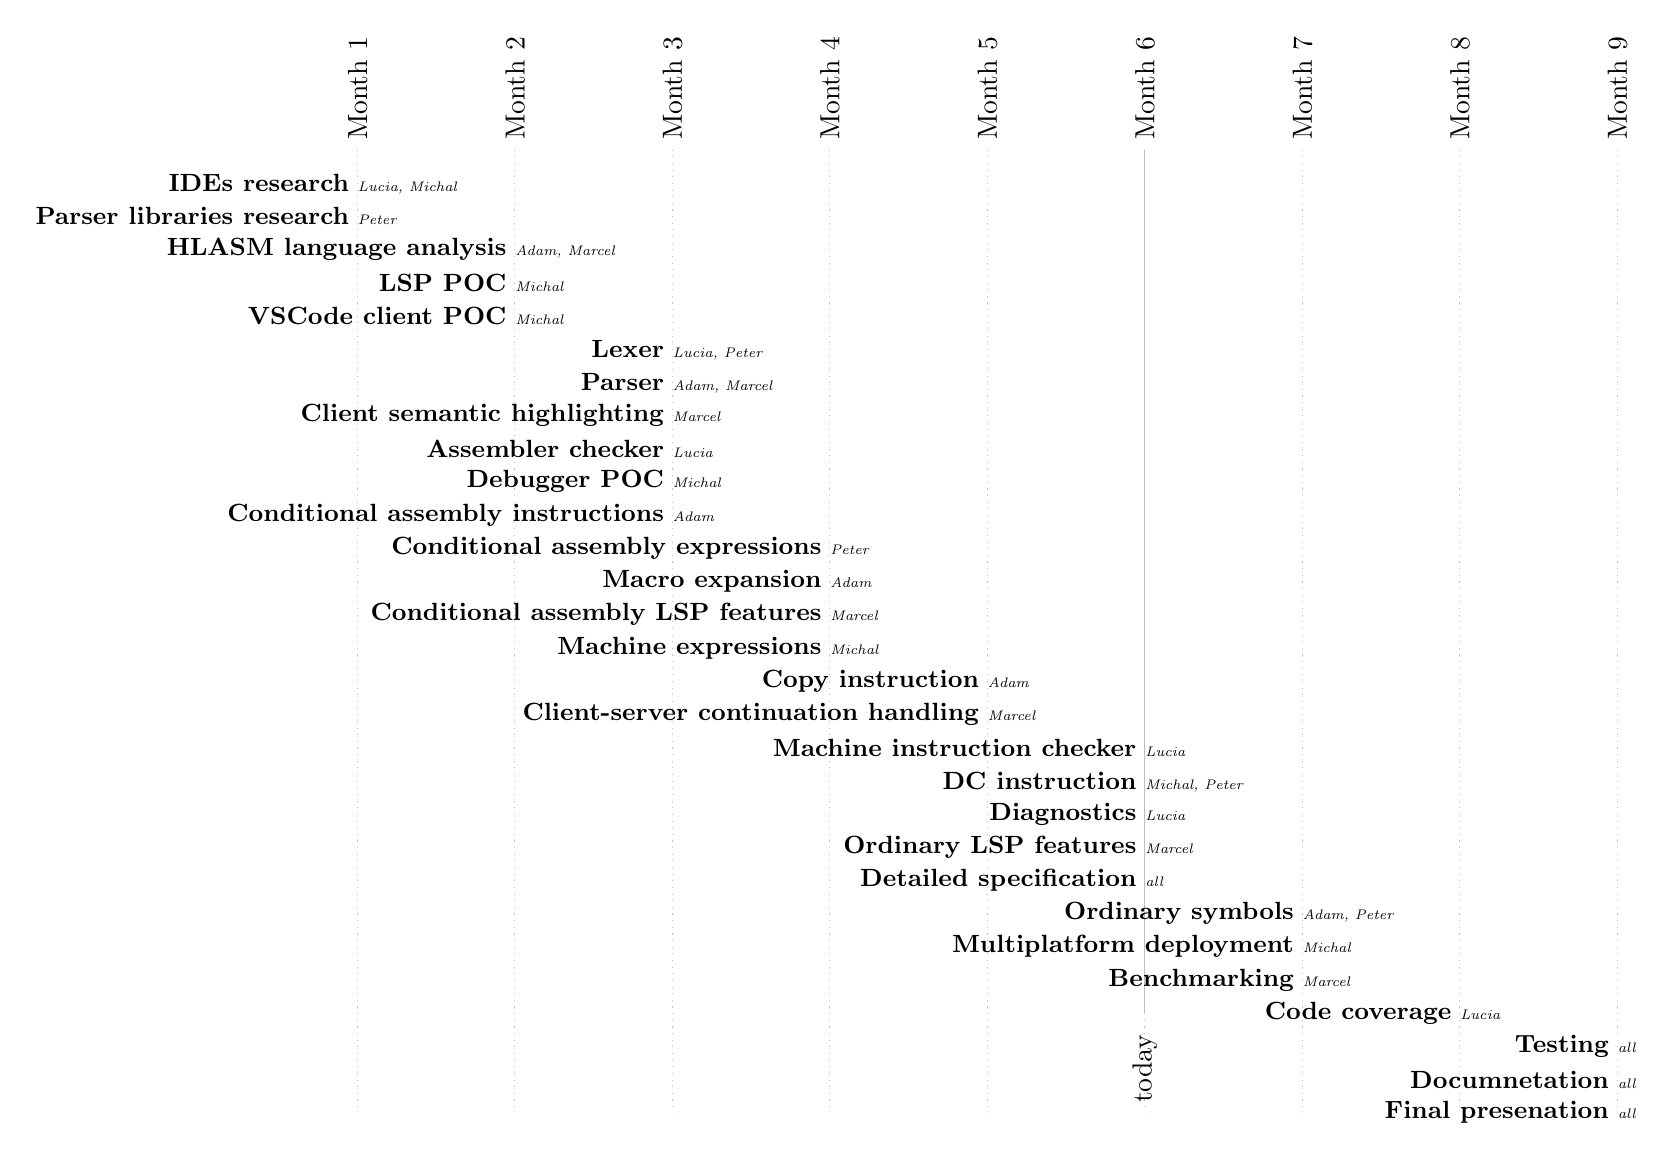
\begin{tikzpicture}
		\foreach \wp in {1,...,30} {
			\coordinate (wp\wp) at (0,\wp * -1.2em);
		};
		\foreach \tim in {1,...,9} {
			\coordinate (t\tim) at (\tim * 2cm,0);
			\node[month] at (t\tim) {Month \tim};
			\draw[dotted, thin, draw=black!25] (t\tim) to (t\tim |- wp29); %sync with previous
		};
		
		
		\draw[draw=black!25] (t6) to (t6 |- wp26); %sync with previous
		\node[month] at (t6|-wp29) {today};
		
		\ganttitem{ider}{t1|-wp1}{IDEs research}{Lucia, Michal};
		\ganttitem{pare}{t1|-wp2}{Parser libraries research}{Peter};
		
		\ganttitem{hlasmla}{t2|-wp3}{HLASM language analysis}{Adam, Marcel};
		\ganttitem{lsppoc}{t2|-wp4}{LSP POC}{Michal}
		\ganttitem{vspoc}{t2|-wp5}{VSCode client POC}{Michal}
		
		\ganttitem{lex}{t3|-wp6}{Lexer}{Lucia, Peter};
		\ganttitem{lex}{t3|-wp7}{Parser}{Adam, Marcel};
		\ganttitem{vspoc}{t3|-wp8}{Client semantic highlighting}{Marcel}
		\ganttitem{lex}{t3|-wp9}{Assembler checker}{Lucia};
		\ganttitem{vspoc}{t3|-wp10}{Debugger POC}{Michal}
		\ganttitem{lex}{t3|-wp11}{Conditional assembly instructions}{Adam};
		
		
		\ganttitem{lex}{t4|-wp12}{Conditional assembly expressions}{Peter};
		\ganttitem{lex}{t4|-wp13}{Macro expansion}{Adam};
		\ganttitem{lex}{t4|-wp14}{Conditional assembly LSP features}{Marcel};
		\ganttitem{lex}{t4|-wp15}{Machine expressions}{Michal};
		
		
		\ganttitem{lex}{t5|-wp16}{Copy instruction}{Adam};
		\ganttitem{lex}{t5|-wp17}{Client-server continuation handling}{Marcel};
		
		
		\ganttitem{lex}{t6|-wp18}{Machine instruction checker}{Lucia};
		\ganttitem{lex}{t6|-wp19}{DC instruction}{Michal, Peter};
		\ganttitem{lex}{t6|-wp20}{Diagnostics}{Lucia};
		\ganttitem{lex}{t6|-wp21}{Ordinary LSP features}{Marcel};
		\ganttitem{lex}{t6|-wp22}{Detailed specification}{all};
		
		
		\ganttitem{lex}{t7|-wp23}{Ordinary symbols}{Adam, Peter};
		\ganttitem{lex}{t7|-wp24}{Multiplatform deployment}{Michal};
		\ganttitem{lex}{t7|-wp25}{Benchmarking}{Marcel};
		
		
		\ganttitem{lex}{t8|-wp26}{Code coverage}{Lucia};
		
		\ganttitem{lex}{t9|-wp27}{Testing}{all};
		\ganttitem{lex}{t9|-wp28}{Documnetation}{all};
		\ganttitem{lex}{t9|-wp29}{Final presenation}{all};
		
		
		\end{tikzpicture}
		\caption{Work packages overview}
		\label{fig:gantt-pokus}
	\end{figure}
\end{landscape}

\iffalse
\newgeometry{a4paper,left=1in,right=1in,top=1in,bottom=1in,nohead}

\begin{landscape}
	\begin{figure}
		\centering
		\begin{ganttchart}[vgrid={draw=none, dotted}, x unit = 1.2cm]{1}{12}
		
		\gantttitlelist{"1. month", "2. month", "3. month"}{4} \\
		\gantttitlelist{1,...,12}{1} \\
		
		\ganttbar{HLASM language analysis (A \& Ma)}{1}{8} \\
		\ganttbar{Parser libraries research (P)}{1}{4}\\
		\ganttbar{IDEs research (L \& Mi)}{1}{4}\\
		
		\ganttbar{LSP POC (Mi)}{5}{8} \\
		\ganttbar{VSCode client POC(Mi)}{5}{8}\\
		\ganttbar{Lexer (L \& P)}{5}{10}\\
		\ganttbar{Parser (A \& Ma)}{5}{12}\\
		
		\ganttbar{Client semantic highlighting (Ma)}{9}{12}\\
		\ganttbar{Assembler checker (L)}{9}{12}\\
		\ganttbar{Debugger POC (Mi)}{9}{12}\\
		\ganttbar{Conditional assembly instructions (A)}{9}{12}\\
		\ganttbar{Conditional assembly expressions (P) $\rightarrow$}{11}{12}\\
		
		
		\end{ganttchart}
    \caption{Tasks for months 1 -- 3}
	\label{fig:gantt1}
	\end{figure}
\end{landscape}


\begin{landscape}
	\begin{figure}
		\centering
		\begin{ganttchart}[vgrid={draw=none, dotted}, x unit = 1.2cm]{1}{12}
			
			\gantttitlelist{"4. month", "5. month", "6. month"}{4} \\
			\gantttitlelist{13,...,24}{1} \\
			\ganttbar{$\rightarrow$ Conditional assembly expressions (P)}{1}{2}\\
			\ganttbar{Macro expansion (A)}{1}{4}\\
			\ganttbar{Conditional assembly LSP features (Ma)}{1}{4}\\
			\ganttbar{Machine expressions (Mi)}{1}{4}\\
			
			\ganttmilestone{Demo presentation}{4}\\
			
			\ganttbar{Machine instruction checker (L)}{1}{12}\\
			\ganttbar{DC instruction (Mi \& P)}{3}{12}\\
			
			\ganttbar{Copy instruction (A)}{5}{8}\\
			\ganttbar{Client-server continuation handling (Ma)}{5}{8}\\
			
			\ganttbar{Diagnostics (L)}{9}{12} \\
			\ganttbar{Ordinary LSP features (Ma)}{9}{12}\\
			\ganttbar{Ordinary symbols (A \& P) $\rightarrow$}{9}{12}
			
			\ganttvrule[vrule offset=0.8]{today}{12}
			
		\end{ganttchart}
		\caption{Tasks for months 4 -- 6}
		\label{fig:gantt2}
	\end{figure}
\end{landscape}

\begin{landscape}
	\begin{figure}
		\centering
		\begin{ganttchart}[vgrid={draw=none, dotted}, x unit = 1.2cm]{1}{12}
			
			\gantttitlelist{"7. month", "8. month", "9. month"}{4} \\
			\gantttitlelist{25,...,36}{1} \\
			
			
			\ganttbar{$\rightarrow$ Ordinary symbols (A \& P)}{1}{4}\\
			\ganttbar{Multiplatform deployment (Mi)}{1}{4}\\
			\ganttbar{Benchmarking (Ma)}{1}{4}\\
			\ganttbar{Code coverage (L)}{1}{8}\\
			
			\ganttbar{Testing (all)}{5}{12}\\
			
			\ganttbar{Documentation (all)}{9}{12}\\
		
			
			\ganttvrule[vrule offset=0.2]{today}{1}
			
		\end{ganttchart}
		\caption{Tasks for months 7 -- 9}
		\label{fig:gantt3}
	\end{figure}
\end{landscape}

\restoregeometry

\fi



